\documentclass[10pt]{article}

\usepackage{polski}
\usepackage{graphicx}
\usepackage{hyperref}
\usepackage{subfigure}
\usepackage[font=footnotesize]{caption}
\usepackage{geometry}
\usepackage{indentfirst}
\usepackage{amsmath}
\usepackage{fancyhdr}


\captionsetup{hypcap=false}
\graphicspath{{images/}}
\newgeometry{tmargin=4cm, bmargin=4cm, lmargin=3.2cm, rmargin=3.2cm} 
\pagestyle{fancy}
\def\nl{\\\hline}

\begin{document}
\begin{titlepage}
  \begin{center}
    \LARGE \textsc{Politechnika Wrocławska}\\
    \vspace*{0.2cm}
    \Large \textsc{Wydział Informatyki i Telekomunikacji}\\  
    \vspace*{0.4cm}
    
\includegraphics[width=0.2\textwidth]{figures/WITlogo.png}\\
    \vspace*{0.2cm}
    \vspace*{2cm}
          
    \centerline{\rule{\textwidth}{1.2pt}}
    \vspace{0.4cm}
    \Huge\textbf{Widzenie komputerowe}
    \centerline{\rule{\textwidth}{1.2pt}}
    \vspace{1cm}
    \LARGE Sprawozdanie z laboratorium\\
    \vspace{3.5cm}
    \textsc{Autor}\\
    \vspace{0.2cm}
    \textbf{Przemysław Barcicki}\\
    \vspace{0.1cm}
    \Large nr albumu: \textbf{260324}\\
    \vspace{0.1cm}
    kierunek: \textbf{Inżynieria systemów}
              
              
          
          
    \vspace*{\fill}
    \Large \textit{07 styczeń 2022}
              
  \end{center}
\end{titlepage}
  
\begin{abstract}
  Zaproponowano własny model sieci neuronowej do segmentacji cyfr na obrazach którego jakość uczenia badano porównując do zmodyfikowanych gotowych sieci \textbf{podobnego} zastosowania wyuczonych dla dużo większego zbioru danych w celu określenia czy lepiej jest modyfikować gotowe modele, czy też od zera uczyć własne. Okazało się, że autorskie rozwiązanie spisało się zdecydowanie lepiej niż pozostałe.
\end{abstract}

\section{Wstęp -- opis problemu}
\label{sec:wstep}

Problem segmentacji obrazów w uczeniu maszynowym w ostatnim czasie stał się bardzo popularny ze względu na możliwości wykorzystania odpowiednio wyuczonych modeli w medycynie czy też w autonomicznych pojazdach. Wspomaganie człowieka w tych obszarach zrewolucjonizowałoby dzisiejszy świat pomagając w szybszych i efektywniejszych diagnozach obrazów medycznych np. pochodzących z rezonansu magnetycznego, ale mogłoby też kompletnie zmienić statystyki bezpieczeństwa na drogach.

Problem segmentacji cyfr na obrazach został już rozwiązany ale zawsze trwają prace nad lepszymi metodami uczenia, lepszymi architekturami sieci oraz lepszymi algorytmami uczenia, aby osiągnać wymaganą celność w dużo szybszym czasie lub z mniejszym nakładem zasobów.

\section{Opis rozwiązania}

\subsection{Dane}

Dane wykorzystywane do uczenia pochodzą z ogólnodostępnego zbioru danych ręcznie pisanych cyfr \verb+MNIST+, które zostały odpowiednio przygotowane do wykorzystania w problemach uczenia maszynowego. Dane wyciągane ze zbioru są przekształcane za pomocą autorskiej biblioteki w języku Python. Każda cyfra jest skalowana oraz obracana o losową wartość. Tak przekształcone cyfry umieszczane są w losowym miejscu na planszy o wielkości $512px\ \times\ 512px$, do której na koniec zostaje dodany losowy szum. Ze względu na to, że kolor cyfry nie ma żadnego znaczenia pozwoliłem sobie pominąć resztę kanałów.

Etykiety do danych również musiały zostać wygenerowane. Korzystano z informacji o miejscu gdzie umieszczono daną cyfrę, z samej przekształconej cyfry oraz etykiety pochodzącej ze zbioru aby stworzyć macierz o wymiarach $(32, 32)$ gdzie zaznaczono przeskalowane cyfry przypisując w tych miejscach $wart_{etykiety} + 1$ (,,tło'' ma wartość 0, zatem ,,0'' ma wartość 1), tak aby dostać etykiety rzadkie.

\begin{center}
  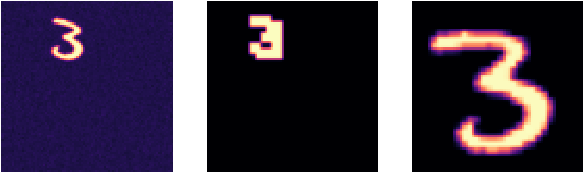
\includegraphics[width=0.7\linewidth]{figures/imagelabel.pdf}
  \captionof{figure}{Przykładowo wygenerowane dane, po lewej znajdują się plansze wejściowe, po środku wygenerowane etykiety, a po prawej cyfra znajdująca się w zbiorze.}
  \label{fig:dane}
\end{center}

\subsection{Sieci}
\label{sec:klasyfikator}

Do celów porównania skorzystano z trzech sieci neuronowych, dwóch gotowych (zmodyfikowanych), \verb+MobileNet+ oraz \verb+EfficientNetB0+, używanych do klasyfikacji zawartości obrazów, każdej z nich w dwóch wariantach. W pierwszym wariancie cała sieć jest w stanie się uczyć, w drugim ,,zamrożonym'', zablokowano możliwość uczenia się warstwom z oryginalnego modelu i uczą się tylko przejściowe warstwy. Trzecia sieć jest autorskim rozwiązaniem i będzie użyta tylko w jednej formie. Łącznie badaniom zostanie podjęte 5 sieci.

\subsubsection{Sieć autorska}
\label{subsec:autorska}

Do porównywania jakości uczenia skorzystano z autorskiej sieci konwolucyjnej, która powstała z mocnej modyfikacji gotowej architektury \verb+YOLOv1+. Cała struktura polega na powtarzających się blokach konwolucyjnych zakończonych warstwą \verb+MaxPooling+ oraz \verb+Dropout+ Poglądową strukturę autorskiej sieci przedstawia rysunek \ref{fig:konwolucyjna_wlasna}. Dokładne listowanie struktury znajduje się na końcu dokumentu w dodatku \ref{app:listowanie}.

\begin{center}
  \centering
  \def\svgwidth{0.9\linewidth}
  \input{figures/nn_ready.pdf_tex}
  \captionof{figure}{Proponowana struktura autorskiej sieci.}
  \label{fig:konwolucyjna_wlasna}
\end{center}

\subsubsection{MobileNet} \label{subsec:mobile}
Sieć MobileNet powstała w celu stosowania gotowej architektury w systemach wbudowanych i mobilnych, aby prezentowały najlepsze wyniki przy zastosowaniu najmniejszej ilości warstw i parametrów.

Wykorzystany gotowy model oryginalnie przyjmuje kolorowe obrazy o wymiarach $224px\ \times\ 224px$, nasze wygenerowane plansze są czarno-białe oraz posiadają wymiary $512px\ \times\ 512px$, zatem do sieci została dodana warstwa skalująca oraz pojedyncza warstwa konwolucyjna tworząca dwa brakujące kanały koloru. Ze względu na inne warstwy końcowe modelu, z architektury sieci zostaje wycięte ostatnich 5 warstw, na którch miejsce lądują warstwy zmieniające wymiary, konwolucyjna zmniejszająca ilość kanałów, oraz wymagana do pracy warstwa \emph{softmax}.

\subsubsection{EfficientNet} \label{subsec:efficient}
Sieć EfficientNet podobnie jak MobileNet \ref{subsec:mobile} powstała aby dawać najlepsze wyniki przy najmniejszym zużyciu zasobów, gdzie badano skalowanie warstw w celu osiągnięci najlepszych wyników.

Ponownie jak wcześniej, gotowa architektura oczekuje obrazów w innej rozdzielczości, a na wyjściu daje szereg pojedynczych neuronów. Zostały zastosowane podobne rozwiązania aby sprowadzić model do odpowiedniej wielkości tak jak przy \ref{subsec:mobile}.


\subsection{Algorytm rozpoznawania}
Jak już wcześniej wspomniano wejściem do sieci jest macierz z cyframi o wymiarach $(512,\ 512,\ 1)$, wyjściem jest macierz o wymiarach $(32,\ 32,\ 11)$ z funkcją aktywacji \emph{softmax} przeprowadzoną względem ostatniego wymiaru.
Pierwsze dwa wymiary definiują przeskalowaną względem wejścia płaszczyzne na której zaznaczone są wyjścia z sieci. Wielkość ostatniego wymiaru wynosi 11, ze względu na potrzebe zaznaczenia 10 klas, (od 0 do 9) oraz jednej dodatkowej na ,,tło'' (tylko dlatego, że skorzystaliśmy z \emph{softmax}).

Dane wyjściowe trafiają do funkcji straty liczącej kategorialną entropię krzyżową. Dodatkowym aspektem analizy jakości sieci jest liczenie tej samej entropii z pominięciem klasy która uwzględnia samo tło w celu oceny rzeczywistej jakości odpowiedzi modelu.


\section{Badania symulacyjne}

\subsection{Cel i plan badania}

Celem badawczym jest określenie efektywności uczenia własnego modelu dla zastosowania segmentacji obrazów w porównaniu do korzystania z gotowych lecz zmodyfikowanych architektur z gotowymi wagami. Badanie będzie polegało na zestawieniu prędkości i efektywności uczenia się modelu korzystając z takich samych ustawień.

\subsubsection{Przyjęte ustawienia}
Każdy model podczas uczenia korzystał z optymalizatora \verb+SGD+ z domyślnymi parametrami prędkości uczenia, z dodatkowym parametrem momentu Nesterova w wysokości 0.9. Jedna epoka składała się z 1000 iteracji o 1 próbce każda. Uczenie kończyło się po 150 epokach.

\subsection{Wyniki eksperymentów} 
Po zakończeniu uczenia, aby szybko okreslić jak odpowiedzi modelu zbliżyły się do wartości oczekiwanych można spojrzeć na wartość funkcji straty. Wykres \ref{plot:loss} przedstawia obie badane przez nas metryki.

\begin{center}
  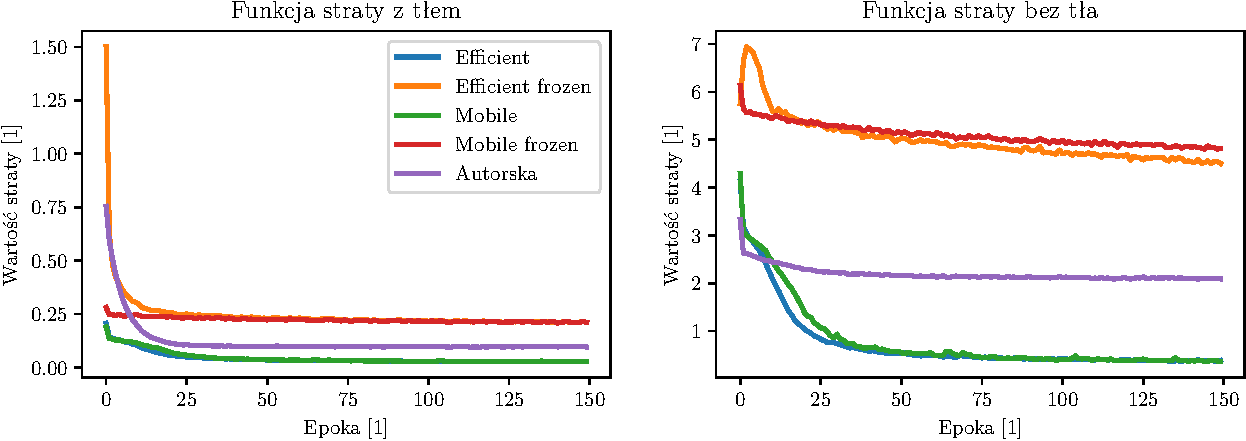
\includegraphics[width=0.9\linewidth]{figures/loss.pdf}
  \captionof{figure}{Wykresy wartości funkcji strat uczonych modeli.}
  \label{plot:loss}
\end{center}

Zauważyć można, że mimo zdecydowanego spowolnienia spadku wartości funkcji straty, wartość straty bez tła cały czas spadała. Linie obu zamrożonych modeli sugerują, że te 150 epok ciągle mogło być za mało, ale zważając na to, jak wysoko ponad zerem się one znajdują, najprawdopodobniej nie spadłyby poniżej 3, nawet po 1000 epokach. Modele zamrożone, osiągnęły wartości blisko zeru bardzo szybko po rozpoczęciu nauki, prawdopodobnie dlatego, że były już wcześniej uczone do rozpoznawania kształtów na obrazach.

\begin{center}
  \begin{tabular}{|c|c|c|c|c|c|}
	\hline
	 &	Efficient &	Efficient frozen &	Mobile &	Mobile frozen &	Own \nl
	$\min\emph{loss}$ &	0.02744 &	0.20855 &	0.02729 &	0.20788 &	0.09523 \nl
	$\min\emph{loss}_{background}$ &	0.35908 &	4.50339 &	0.36454 &	4.80074 &	2.08145 \nl
\end{tabular}
  \captionof{table}{Minimalne wartości funkcji strat dla każdego modelu.}
  \label{table:loss}
\end{center}

% Zważając na wartości funkcji strat można wstępnie określić kolejność jakości modeli.
% \begin{equation*}
%     \text{Efficient} > \text{Mobile} > \text{Own} > \text{Efficient Frozen} > \text{Mobile Frozen}
% \end{equation*}

\noindent
Następnym krokiem będzie wizualne zbadanie predykcji każdego z modeli.

\begin{center}
  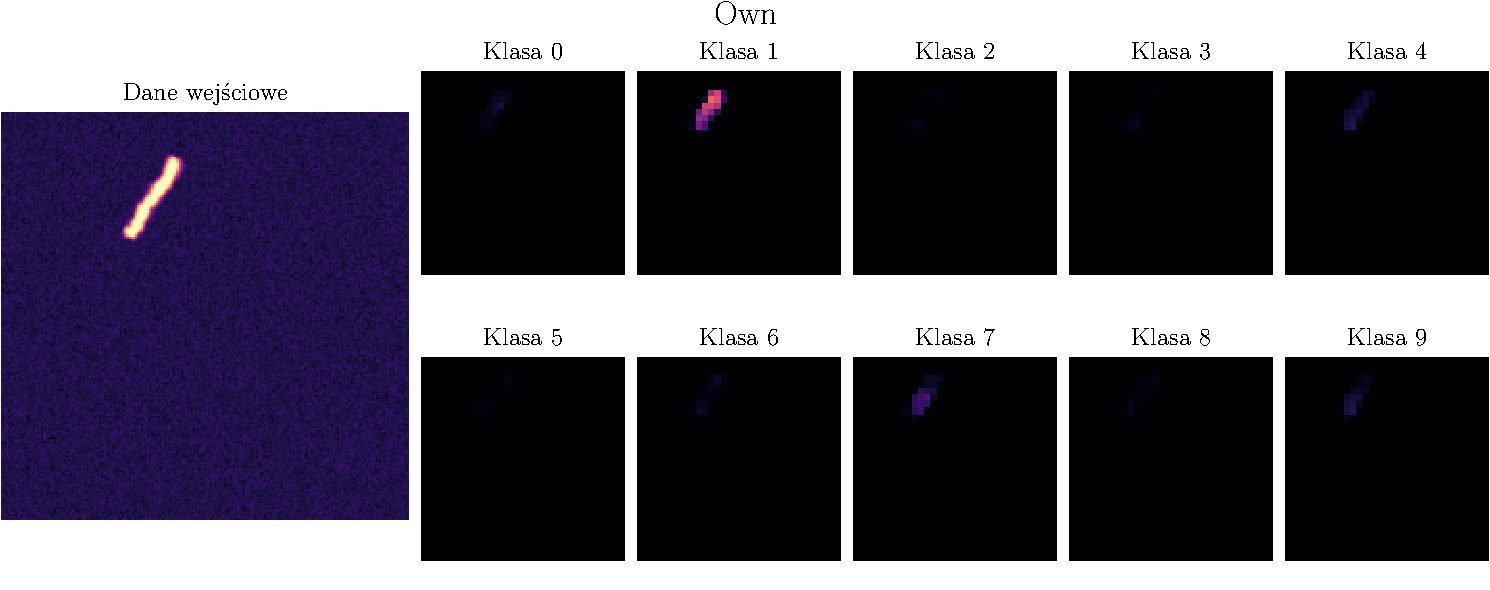
\includegraphics[width=0.9\linewidth]{figures/own.pdf}
  \captionof{figure}{Predykcja sieci autorskiej.}
  \label{fig:own_resp}
\end{center}

\begin{center}
  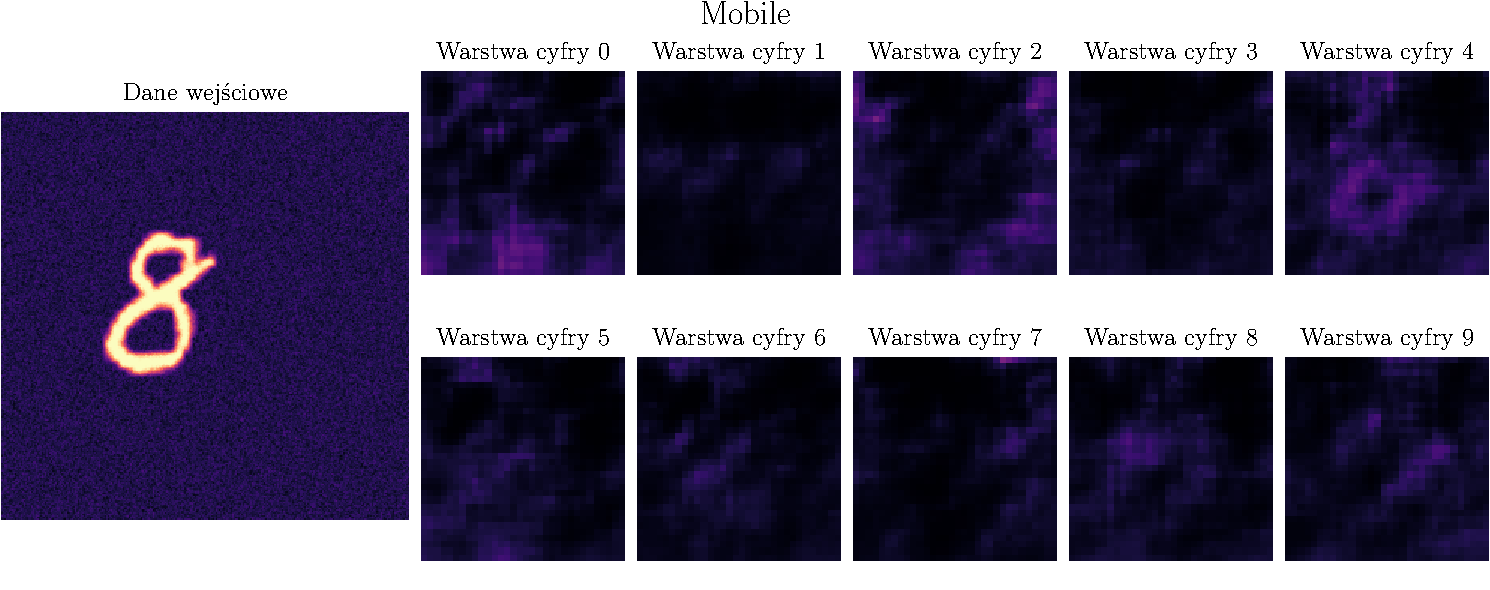
\includegraphics[width=0.9\linewidth]{figures/mobile.pdf}
  \captionof{figure}{Predykcja sieci MobileNet.}
  \label{fig:mobile_resp}
\end{center}

\begin{center}
  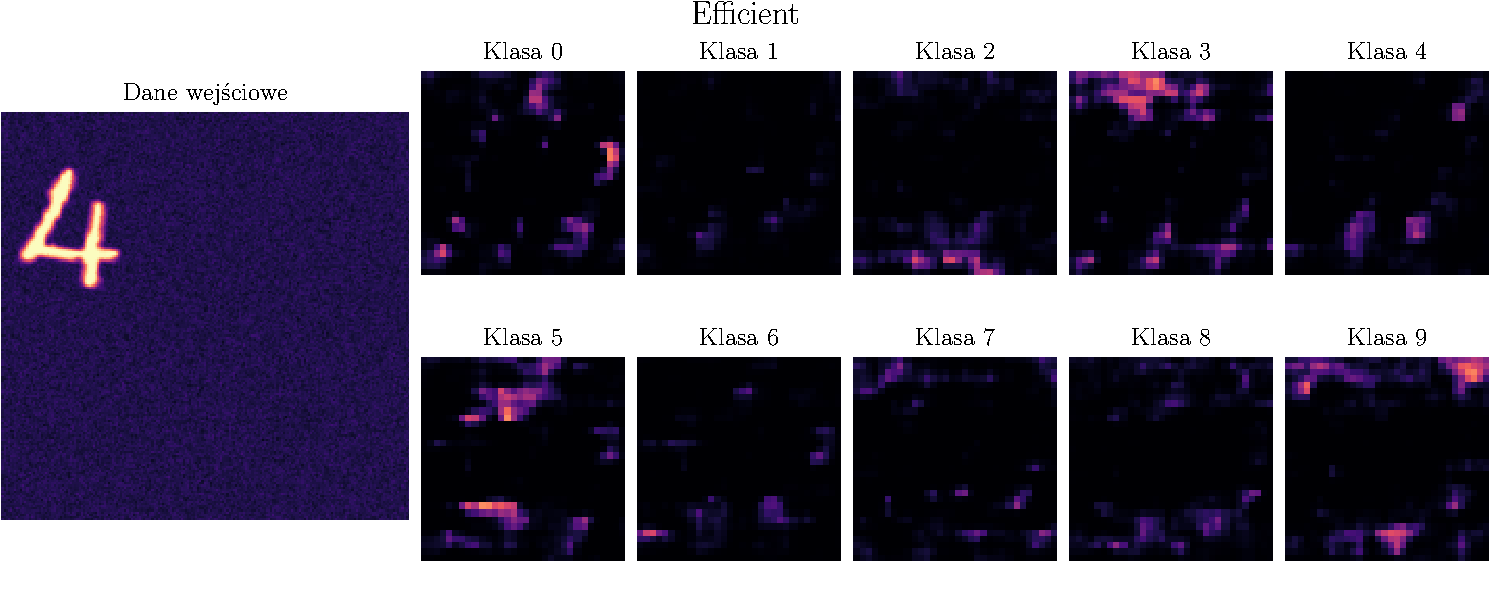
\includegraphics[width=0.9\linewidth]{figures/efficient.pdf}
  \captionof{figure}{Predykcja sieci EfficientNet.}
  \label{fig:efficient_resp}
\end{center}

\begin{center}
  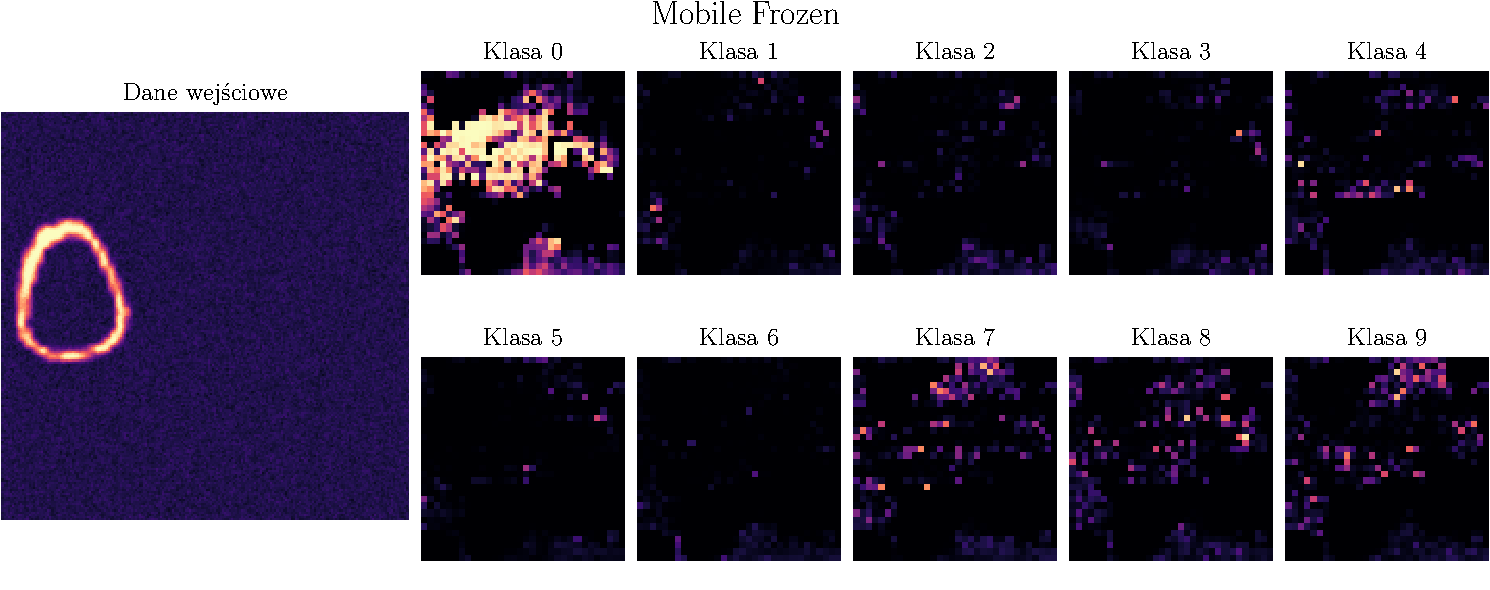
\includegraphics[width=0.9\linewidth]{figures/mobile_frozen.pdf}
  \captionof{figure}{Predykcja zamrożonej sieci MobileNet.}
  \label{fig:mobile_frozen_resp}
\end{center}

\begin{center}
  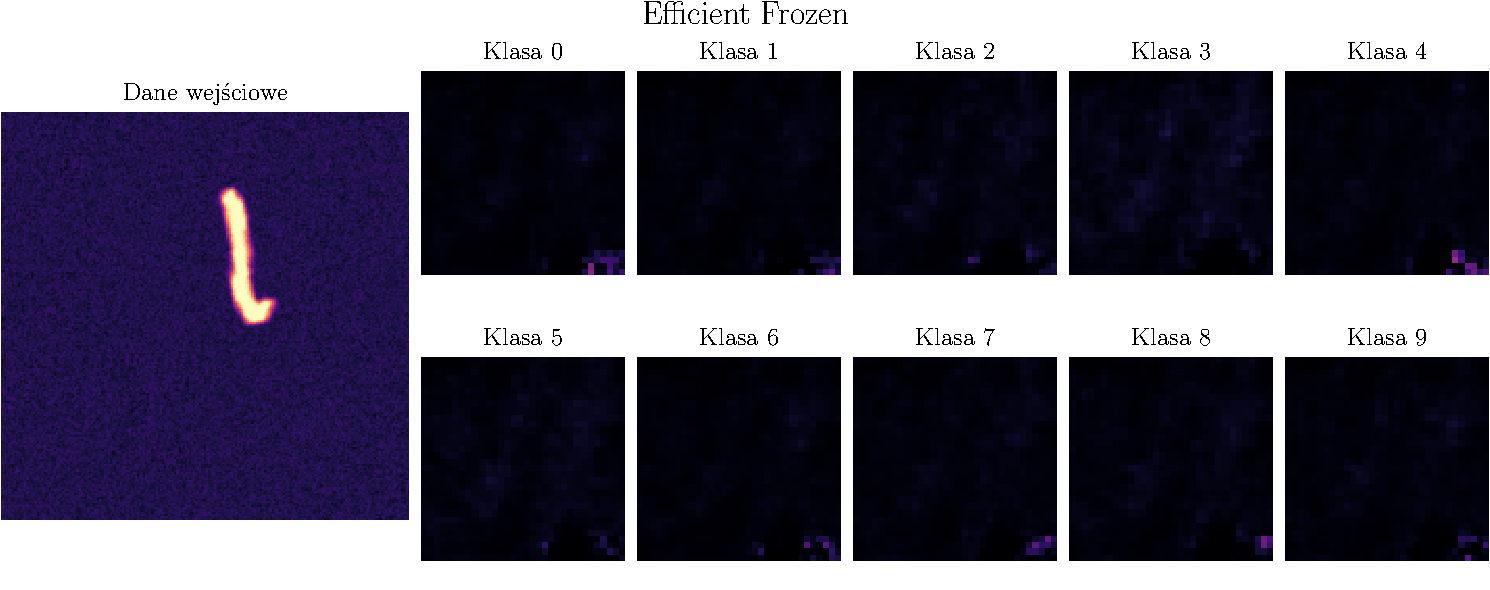
\includegraphics[width=0.9\linewidth]{figures/efficient_frozen.pdf}
  \captionof{figure}{Predykcja zamrożonej sieci EfficientNet.}
  \label{fig:efficient_frozen_resp}
\end{center}

\newpage
Okazuje się, że sieci które objawiały się najlepszymi wynikami uczenia (\ref{subsec:efficient}, \ref{subsec:mobile}) nie dają równie zadowalających efektów wizualnie. Widać różnice między zwykłymi i zamrożonymi odpowiednikami tych sieci, co sugerowałoby, że jakaś nauka zachodziła, lecz nie dała ona żadnych efektów. Sieć autorska widocznie zaznacza na poszczególnych klasach zarys odpowiedniej wartości, jednak większość odpowiedzi znajduje się w odpowiednim miejscu (widać pewien lekki zarys w oknie odpowiadającym liczbie 7 ze względu na dużą część wspólną pisanej 1 i 7).

\section{Wnioski}
Stworzenie własnej sieci która od początku miała za zadanie rozpoznawać cyfry na planszy okazało się dużo bardziej efektywne od modyfikowania istniejących sieci które, albo błądziły ze swoimi odpowiedziami i próbowały ,,oszukać'' funkcję straty, albo nie nauczyły się niczego. Prawdopodobnie istnieje możliwość transplantacji warstw między modelami tak aby dawały one bardzo zadawalające efekty, ale wymaga to bardzo dobrej znajomości narzędzi, oraz wiedzy na temat tego czego i jak tak naprawde się ta sieć uczy.

\begin{thebibliography}{9}
  \bibitem{bib:yolo}
  Joseph Redmon and Santosh Divvala and Ross Girshick and Ali Farhadi
  You Only Look Once: Unified, Real-Time Object Detection (2015)
  \bibitem{bib:efficientnet}
  Andrew G. Howard and Menglong Zhu and Bo Chen and Dmitry Kalenichenko and Weijun Wang and Tobias Weyand and Marco Andreetto and Hartwig Adam
  MobileNets: Efficient Convolutional Neural Networks for Mobile Vision Applications (2017) 
  \bibitem{bib:mobilenet}
  Mingxing Tan and Quoc V. Le
  EfficientNet: Rethinking Model Scaling for Convolutional Neural Networks (2019)
\end{thebibliography}

\appendix

\section{Listowanie struktury sieci}
\label{app:listowanie}
\begin{center}
  \begin{tabular}{|c|c|c|}
    \hline
    Typ warstwy     & Wielkość wyjściowa  & Ilość parametrów \nl
    Conv2D          & $(512,\ 512,\ 32)$  & 2080    \nl
    MaxPooling2D    & $(256,\ 256,\ 32)$  & 0       \nl
    Conv2D          & $(256,\ 256,\ 64)$  & 8256    \nl
    MaxPooling2D    & $(128,\ 128,\ 64)$  & 0       \nl
    Conv2D          & $(128,\ 128,\ 32)$  & 2080    \nl
    Conv2D          & $(128,\ 128,\ 64)$  & 8256    \nl
    Conv2D          & $(128,\ 128,\ 64)$  & 4160    \nl
    Conv2D          & $(128,\ 128,\ 128)$ & 32896   \nl
    MaxPooling2D    & $(64,\ 64,\ 128)$   & 0       \nl
    Dropout         & $(64,\ 64,\ 128)$   & 0       \nl
    Conv2D          & $(64,\ 64,\ 64)$    & 8256    \nl
    Conv2D          & $(64,\ 64,\ 128)$   & 32896   \nl
    Conv2D          & $(64,\ 64,\ 128)$   & 16512   \nl
    Conv2D          & $(64,\ 64,\ 256)$   & 131328  \nl
    MaxPooling2D    & $(32,\ 32,\ 256)$   & 0       \nl
    Dropout         & $(32,\ 32,\ 256)$   & 0       \nl
    Conv2D          & $(32,\ 32,\ 256)$   & 65792   \nl
    Conv2D          & $(32,\ 32,\ 128)$   & 131200  \nl
    Conv2D          & $(32,\ 32,\ 64)$    & 8256    \nl
    Conv2D          & $(32,\ 32,\ 32)$    & 2080    \nl
    Dropout         & $(32,\ 32,\ 32)$    & 0       \nl
    Conv2DTranspose & $(32,\ 32,\ 11)$    & 8811    \nl
    Reshape         & $(32,\ 32,\ 11)$    & 0       \nl
    Softmax         & $(32,\ 32,\ 11)$    & 0       \nl
\end{tabular}
\end{center}
% \footnote{Wizualizacja wygenerowana dzięki narzędziu \url{http://alexlenail.me/NN-SVG/LeNet.html}}.
% Nie byłem w stanie tego wrzucić wyżej, gdzie jest ten obrazek, bo mi nie działał footnote :(

\section{Dodatek}
Kody źródłowe umieszczone zostały w repozytorium GitHub:

\noindent \url{https://github.com/krzesu0/widzenie-komputerowe-projekt}.


\end{document}